\section{Leptons reconstruction and identification}\label{sec:leptonID}

\subsection{Muon reconstruction and identification}\label{sec:muID}
Muons produced at the collision point can go through the entire detector with a negligible energy loss, reaching the detector outermost part where the muon chambers are installed (see Sec.~\ref{sec:muonsyst}). Muons interact through ionization with the layers of the silicon tracker, which is able to reconstruct their tracks (\emph{tracker track}). The muon tracks are also reconstructed using the muon system (\emph{standalone muon track}). Based on these objects, two reconstruction approaches are used~\cite{Chatrchyan:2012xi}: in the first method (outside-in), for each standalone muon track a tracker track is searched for by extrapolating the two tracks to a common surface. If a match is found, the hits associated to the two tracks are fitted together giving rise to a \emph{Global Muon}. The second approach (inside-out) consists in considering all tracker tracks with $\pt > 0.5$\,\GeV as potential muon candidates. These tracks are extrapolated to the muon system taking into account the magnetic field, the expected energy losses and the multiple scattering in the detector material. If at least one muon segment (a short track stub made of DT or CSC hits) matches the extrapolated tracks, the corresponding tracker track is identified as a \emph{Tracker Muon}.

The matching with the muon system improves significantly the muon \pt resolution that can be obtained from the tracker only, especially in the region with $\pt > 200$\GeV, as shown in Fig.~\ref{fig:muptres}. 
\begin{figure}[htb]
\centering
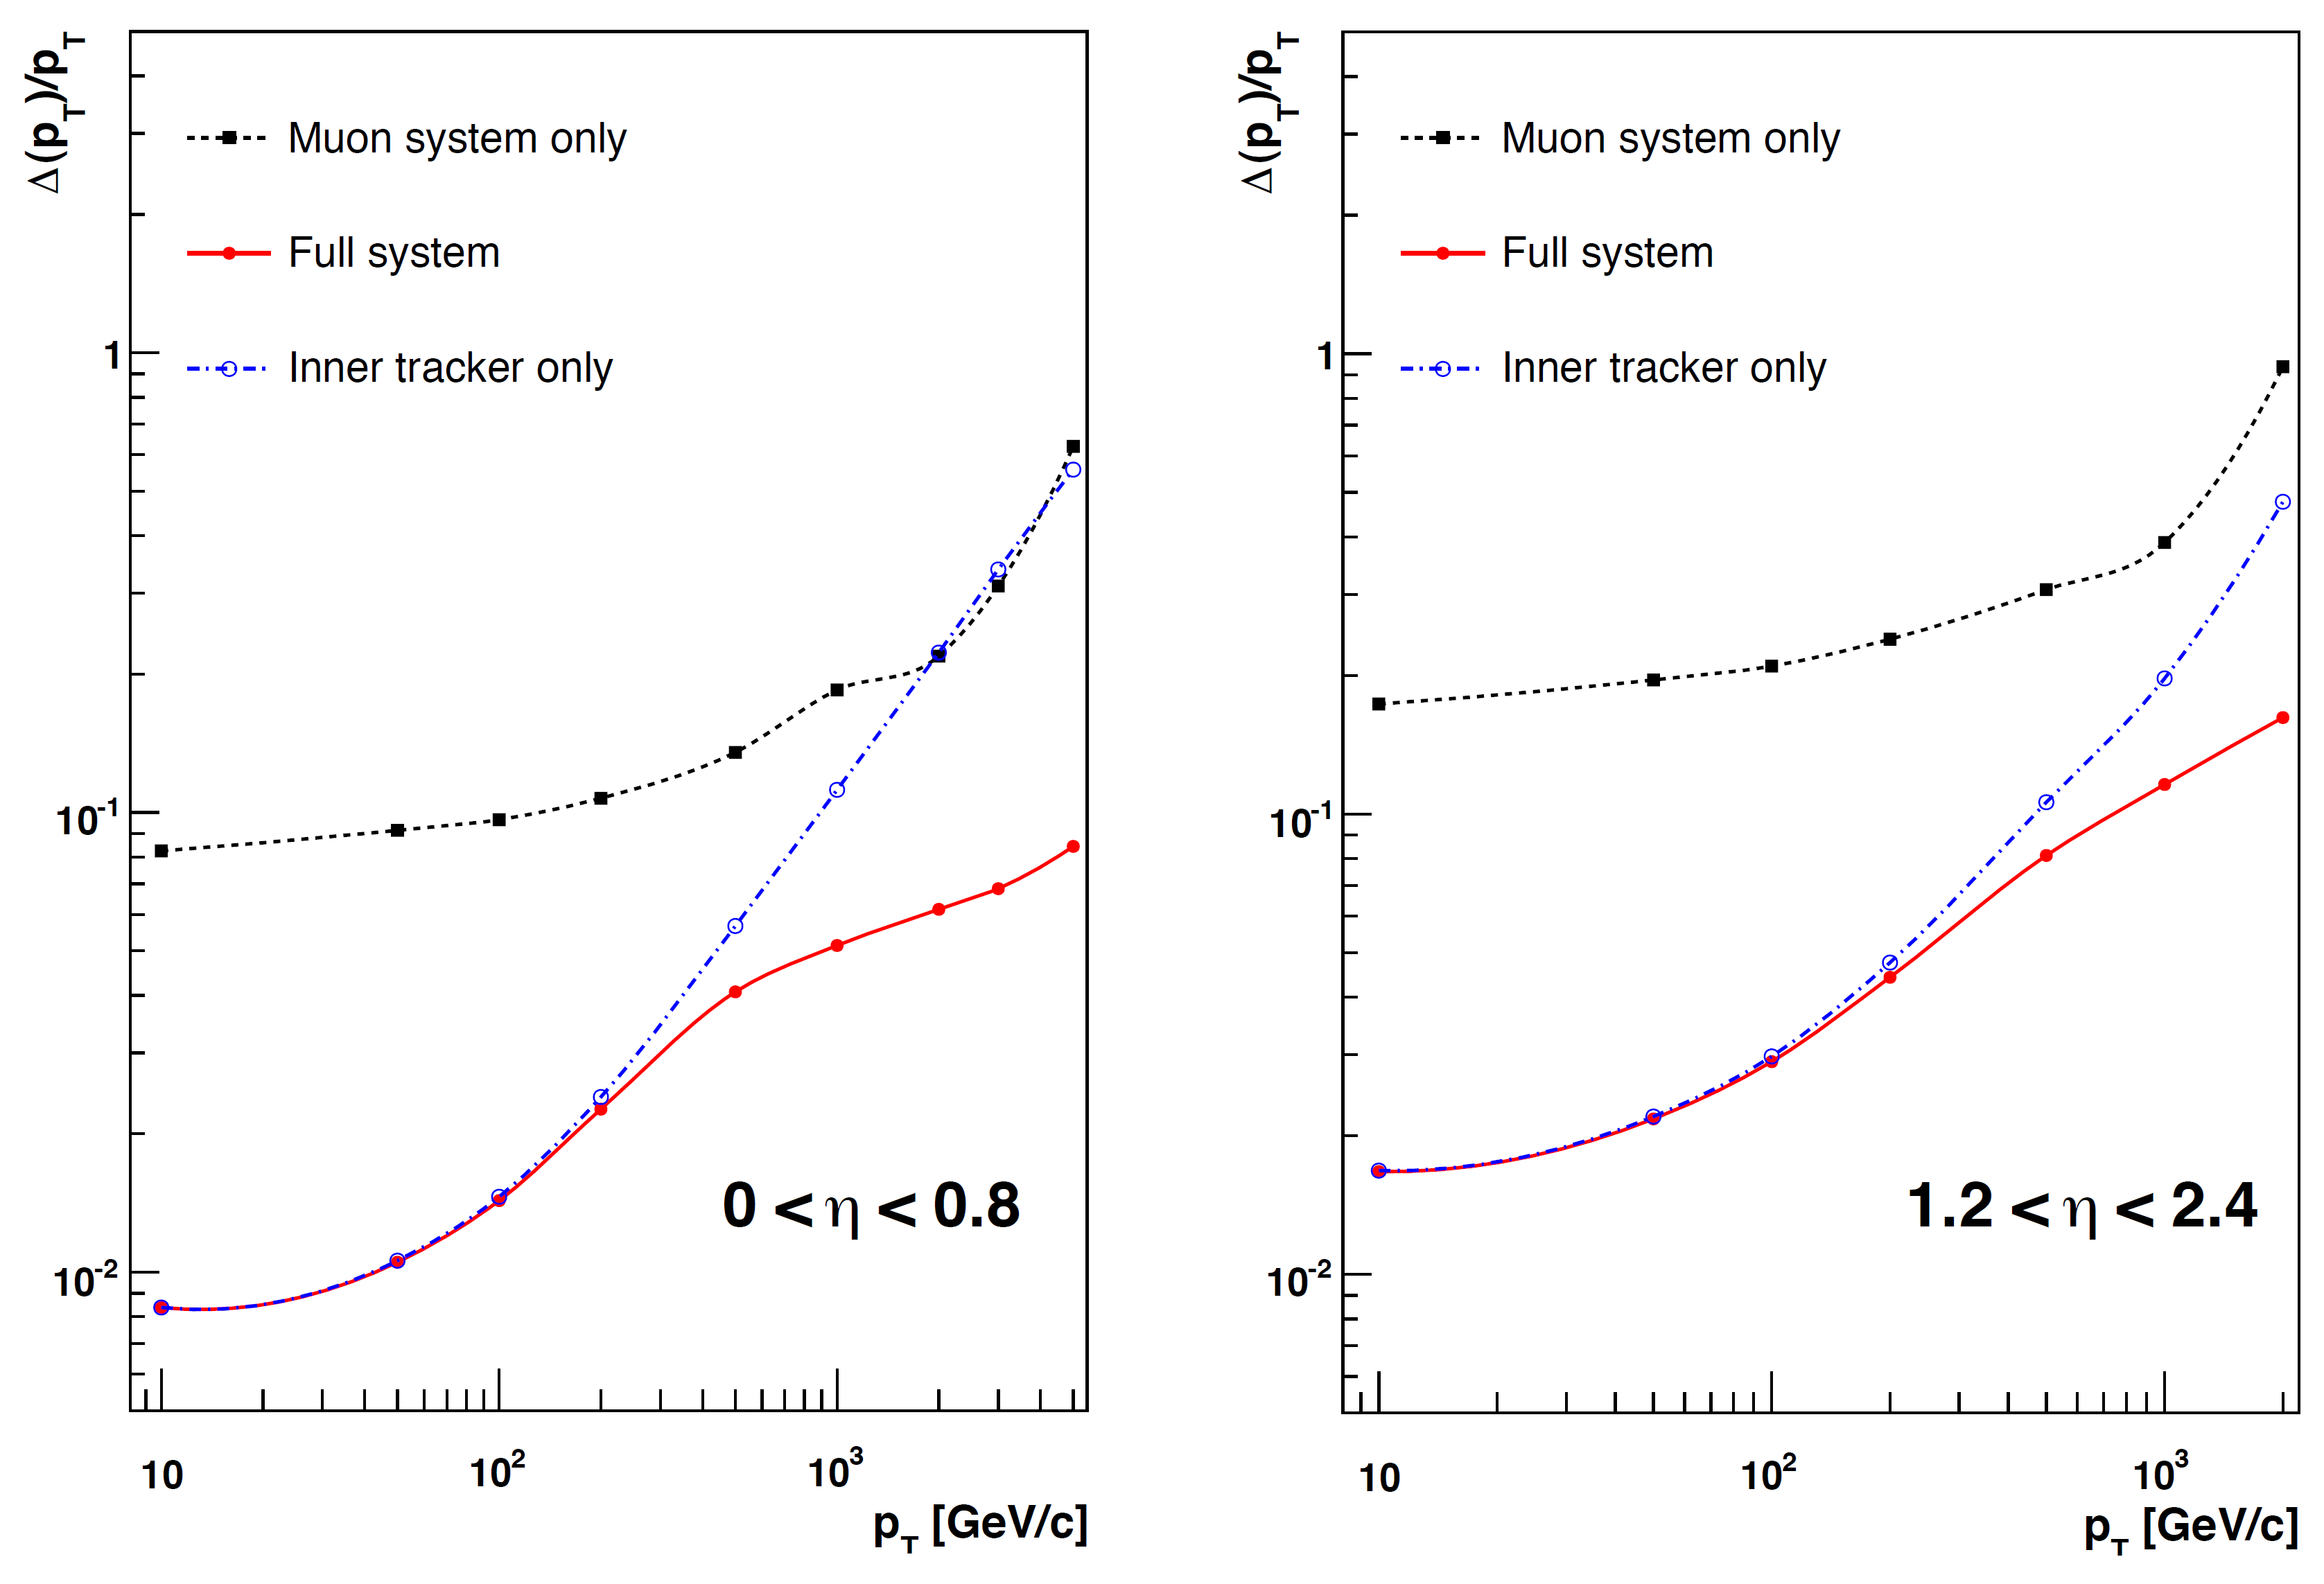
\includegraphics[width=0.6\textwidth]{images/muptres.png}
\caption{Muon \pt resolution as a function of the muon \pt in the barrel (left) and in the endcap (right) region. The resolution is provided for the measurement using the tracking system or the muon system only, as well as for the combination of the two methods.}\label{fig:muptres}
\end{figure}

Depending on the physics analysis, different muon definitions can be used by changing the selection on the muon identification variables, hence balancing between the muon identification efficiency and purity. The most widely used definition in physics analyses at CMS is the so-called \emph{Tight muon selection}\footnote{Small variations with respect to this baseline definition are adopted by the specific analyses.}. This selection requires the muon candidate to be reconstructed as a Global Muon and identified by the PF algorithm. The fit of the global track, which is required to include muon segments in at least two muon stations (this implies that the muon is also reconstructed as a Tracker Muon), must have a $\chi^2/d.o.f.$ less than 10 and use more than 10 inner tracker hits. The transverse impact parameter with respect to the primary vertex is required to be $|d_{xy}|<2$\,mm, significantly reducing the rate of muons from in flight decays, i.e. non-prompt muons. The requirements defining the Tight Muon identification are summarized in Table~\ref{tab:tightmuon}.

\begin{table}[htb]
\caption{Summary of the muon identification variables and the corresponding selections commonly used by physics analyses.}\label{tab:tightmuon}
\centering
\begin{tabular}{lc}
\toprule
Observable & Selection \\
\midrule
Is Global Muon & true \\
Is PF muon & true \\
Tracker layers with valid hits & $>5$ \\
Number of valid pixel hits & $>0$ \\
Number of valid muon hits & $>0$ \\
Number of matched muon stations & $>1$ \\
$\chi^2/d.o.f.$ & $<10$ \\
$d_{xy}(PV)$ & $< 0.2$\,cm \\
$d_{z}(PV)$ & $< 0.5$\,cm \\
\bottomrule
\end{tabular}
\end{table}

Another selection which is optimised for low-\pt muons coming from in flight decays is called \emph{Soft-Muon selection}. This selection requires the muon to be reconstructed as a Tracker Muon with additional loose cuts on the transverse and longitudinal impact parameters. This selection is commonly used to identify muons coming from B hadron decays.

\subsection{Muon isolation}
The isolation is one of the most powerful requirements to select prompt muons, as the ones produced by W or Z boson decays, and to reject muons produced by in flight decays. Indeed, prompt muons are expected to be isolated in the event, differently to non-prompt muons that are generally produced within jets and characterized by many nearby particles.

Muons commonly used to reconstruct the W or Z boson decays are thus required to pass an isolation requirement, which includes a pile-up mitigation correction called ``$\Delta\beta$ correction''. This correction is needed to obtain a robust isolation definition that is less sensitive to the pile-up contribution. Indeed, simultaneous interactions manifest themselves as a mean energy deposited over all the detector acceptance that is not due to particles produced in the primary event, thus spoiling the isolation measurement. The relative isolation variable, usually called \emph{PF relative isolation}, is defined as follows:
\begin{equation}\label{eq:isomu}
I^{rel}_{\Delta\beta} = \left[  \sum_{ChH}\pt + max\left(0, \sum_{NH}\pt + \sum_{Ph}\pt - 0.5\sum_{ChHPU}\pt    \right)  \right]/\pt^\mathrm{muon} \quad .
\end{equation}

The sums in Eq.~\eqref{eq:isomu} are performed in a cone of radius $\Delta R < 0.4$ around the muon direction. The $ChH$ subscript refers to charged hadrons, $NH$ to neutral hadrons, $Ph$ to photons and $ChHPU$ to charged hadrons not arising from the primary vertex.

The cut applied on the isolation variable is analysis dependent, but a common value is $I^{rel}_{\Delta\beta} < 0.15$.

A different isolation definition is called \emph{Tracker relative isolation}, $I^{rel}_{trk}$, which is calculated as the scalar sum of all the \pt of the tracker tracks reconstructed inside a cone of radius $\Delta R < 0.3$ centred on the muon track direction.

\subsection{Muon momentum scale and resolution}
The measurement of the muon \pt is sensitive to the alignment of the tracker and muon chambers, material composition and distribution inside the detector and to the knowledge of the magnetic field produced by the solenoid. The imperfect knowledge of the magnetic field and the effect of the material distribution introduce a relative bias in the muon \pt that is generally independent on the \pt itself, while the effect of the alignment is known to produce a bias that increases linearly with the \pt.

Different methods are used to estimate the muon \pt scale and resolution effects and to determine the corresponding uncertainties depending on the \pt range. At low and intermediate \pt ($< 100$\,\GeV), the dimuon events arising from the $\mathrm{J/\Psi}$ and Z resonance decays are used to correct the \pt scale and to measure the \pt resolution. In the high \pt regime, the muon \pt scale and resolution are instead measured using cosmic ray muons. One of the methods that is commonly used in the intermediate \pt range is the \emph{MuScleFit} (Muon momentum Scale calibration Fit), which provides the muon \pt scale corrections by fitting the Z boson mass peak in data and simulation. These corrections are meant to recover the bias of the Z mass peak with respect to the $\eta$ and $\phi$ coordinates of the muon. After applying these corrections, the relative \pt resolution ($\sigma(\pt)/\pt$) is measured as a function of $\eta$ and $\phi$ and is found to be on average of the order of 2\% in the barrel and up to 6\% in the endcaps, for muon \pt below 100\,\GeV.

\subsection{Electron reconstruction and identification}\label{sec:eleIdIso}

The electron reconstruction is based on the combination of tracker and ECAL information. The reconstruction technique starts by measuring the energy deposits in ECAL by electrons, which form a ``supercluster''. A supercluster is a group of one or more ECAL clusters associated using an algorithm that takes into account the characteristic shape of the energy deposited by electrons emitting \emph{bremsstrahlung} radiation in the tracker material. The supercluster shape is characterized by a narrow width profile in the $\eta$ coordinate spread over the $\phi$ direction. The superclusters are matched to tracks reconstructed in the tracker with the GSF algorithm in order to obtain an electron candidate. An additional reconstruction method, described in details in Refs.~\cite{CMS-PAS-EGM-10-004,Khachatryan:2015hwa}, is instead seeded by electron tracks reconstructed in the inner tracker layers.

Several strategies are used in CMS to identify prompt isolated electrons (characteristic of the signal processes of interest), and to separate them from background sources, mainly originating from photon conversions, jets misidentified as electrons, or electrons from semileptonic decays of b and c quarks. In order to achieve a good discrimination, several identification variables are used:
\begin{itemize}
\item $\Delta\eta_\mathrm{trk,SC}$ and $\Delta\phi_\mathrm{trk,SC}$: the variables measuring the spatial matching between the track and the supercluster in the $\eta$ and $\phi$ coordinates, respectively;
\item $\sigma_{i\eta,i\eta}$: a variable related to the calorimeter shower shape, measuring the width of the ECAL supercluster along the $\eta$ direction computed for all the crystals in the $5
\times 5$ block of crystals centred on the highest energy crystal of the seed supercluster;
\item $H/E$: the ratio between the energy deposited in the HCAL tower behind the ECAL seed and the supercluster seed energy;
\item $|1/E - 1/p|$: the difference of the inverse of energy $E$ measured in ECAL and the inverse of momentum $p$ measured in the tracker;
\item the number of missing hits in the back-propagation of the track to the interaction point;
\item $d_{xy}$ and $d_z$: the transverse and longitudinal impact parameters with respect to the primary vertex.
\item a photon conversion veto ($\gamma \to \mathrm{e^+ e^-}$) based on the primary vertex measurement.
\end{itemize}

Different working points are provided by CMS corresponding to different selections on the previously defined variables. One of the common working points used by several physics analyses, as the \hww analyses described in Chapters~\ref{chap4}, \ref{chap5} and \ref{chap6}, is the ``tight working point'', summarised in Table~\ref{tab:tightele}.

\begin{table}[htb]
\caption{Electron identification selections corresponding to the tight working point.}\label{tab:tightele}
\centering
\begin{tabular}{lcc}
\toprule
\multirow{2}{*}{Variable} & \multicolumn{2}{c}{Selection}\\
 & $|\eta_\mathrm{SC}|\leq 1.479$ & $1.479 < |\eta_\mathrm{SC}| \leq 2.5$ \\
\midrule
$\sigma_{i\eta,i\eta}$ & 0.01 & 0.028 \\
$|\Delta\eta_\mathrm{trk,SC}|$ & 0.009 & 0.007 \\
$|\Delta\phi_\mathrm{trk,SC}|$ & 0.03 & 0.09 \\
$H/E$ & 0.06 & 0.06 \\
$|1/E - 1/p|$ & 0.012 & 0.010 \\
$|d_{xy}|$ & 0.011\,cm & 0.035\,cm\\
$|d_{z}|$ & 0.047\,cm & 0.42\,cm\\
missing inner hits & $\leq 2$ & $\leq 1$\\
conversion veto & yes & yes \\
\bottomrule
\end{tabular}
\end{table}

\subsection{Electron isolation}
Selected electrons are required to pass an isolation requirement that includes a pile-up mitigation correction based on the electron effective catchment area, which is different in different $\eta$ ranges. The isolation variable is given by the following formula:
\begin{equation}
I^{rel}_{EA~corrected} = \left[ \sum_{ChH}\pt + max\left( 0, \sum_{Ph}\pt + \sum_{NH}\pt - \rho EA \right) \right]/\pt^\mathrm{electron} \,
\end{equation}

\noindent where $ChH$ refers to charged hadrons, $Ph$ to photons, $NH$ to neutral hadrons, $\rho$ is the energy density due to pile-up events, $E$ is the energy and $A$ is an effective area. The sums are performed inside a cone of radius $\Delta R < 0.4$ around the electron direction. The selection applied on this variable for the tight working point is $I^{rel}_{EA~corrected} < 0.04$.

\subsection{Electron momentum scale and resolution}
The electron momentum is estimated using a combination of the tracker and ECAL measurements. The ECAL energy response is calibrated before making the combination of the two measurements. Before doing the clustering, the energy response in individual crystals is calibrated and a correction factor is applied to take into account effects as energy leakage or changes in the crystal transparency induced by radiation~\footnote{The continuous monitoring of the crystals transparency is achieved by a laser-monitoring system.}. Then the supercluster energy is also corrected using an MVA technique, selecting $\mathrm{Z\to e^+ e^-}$ events in data and comparing to simulation. A detailed description of the techniques used to estimate the electron scale and resolution and the associated uncertainties is given in Ref.~\cite{Khachatryan:2015hwa}.



\subsection{Lepton identification and isolation efficiency}\label{sec:lepIdIsoEff}
The efficiency related to the identification and isolation selections applied to muons and electrons is generally estimated both in data and simulation, and simulated events are corrected for the observed differences by means of a scale factor ($SF$), defined as the ratio of the efficiency measured in data ($\varepsilon_\mathrm{data}$) and simulation ($\varepsilon_\mathrm{MC}$), i.e. $SF = \varepsilon_\mathrm{data}/\varepsilon_\mathrm{MC}$.

The identification and isolation efficiencies are measured using a Tag and Probe technique. 
The Tag and Probe technique is a method to estimate the efficiency of a selection on data. In can be applied whenever one has two objects in a given event by using one of the two, the \tg{}, to identify the process of interest and the second, the \probe{}, to actually measure the efficiency of the selection being studied.
Concerning the electron and muon case, the Tag and Probe method uses a known mass resonance (e.g. $\mathrm{J/\Psi}$, Z) to select particles of the desired type, and probe the efficiency of a particular selection criterion on these particles. In general the \tg{} is an object that passes a set of very tight selection criteria designed to isolate the required particle type. Tags are often referred to as a ``golden'' electrons or muons and the fake rate for passing tag selection criteria should be very small. A generic set of the desired particle type, the \probe{} (defined with potentially very loose selection criteria) is selected by pairing these objects with tags such that the invariant mass of the combination is consistent with the mass of the resonance. Combinatoric backgrounds may be eliminated through any of a variety of background subtraction methods such as fitting, or sideband subtraction. The definition of the probe objects depend on the specifics of the selection criterion being examined. The simple expression to get the efficiency $\varepsilon$ as a function of \pt and $\eta$ is given below:
\begin{equation}\label{eq:tagprobe}
\varepsilon(\pt,\eta) = \frac{ N^\mathrm{probe}_\mathrm{pass}}{N^\mathrm{probe}_\mathrm{pass} + N^\mathrm{probe}_\mathrm{fail}}
\end{equation}

For the estimation of the electron or muon identification efficiency, the tag is chosen to be a well identified and isolated electron or muon, while the probe is chosen as an electron or muon identified with loose selections. The invariant mass of the \tp pair is required to be within a window around the Z boson mass (the effect of changing the Z mass window is included as a systematic uncertainty). After that, the probe is required to pass the identification selections discussed before for electrons and muons, and the efficiency is computed both in data and simulation. A scale factor is then calculated by taking the ratio of the two efficiencies and applied to reweight simulated events.

There are two methods to measure the efficiencies: the counting method consists in simply computing the ratio of probe events that pass the selections and total number of probe events, as shown in Eq.~\eqref{eq:tagprobe}. This method can be used when the tag requirement selects a very pure set of events, with a small background contribution. The other approach is the fitting method, which is used when the background contamination is not negligible. In this latter case, which represents the commonly used method for estimating the lepton identification and isolation efficiencies, the invariant mass distribution of the tag-probe pair for signal and background is fitted choosing proper functions. The signal plus background fit is performed simultaneously in two categories, corresponding to events in which the probe lepton passes or fails the identification requirements, and separately in bins of $\eta$ and \pt.

A similar approach is used to estimate the lepton isolation efficiency, requiring the probe lepton to pass the isolation requirements instead of the identification ones and calculating the corresponding scale factor.

The electron identification and isolation efficiency and the scale factor are shown in Fig.~\ref{fig:eleIdIso}, corresponding to the selections described in Sec.~\ref{sec:eleIdIso}, for events of interest for a typical physics analysis of the \hwwllnn channel (in particular the analyses described in Chapters~\ref{chap5} and \ref{chap6}).

\begin{figure}[htb]
\centering
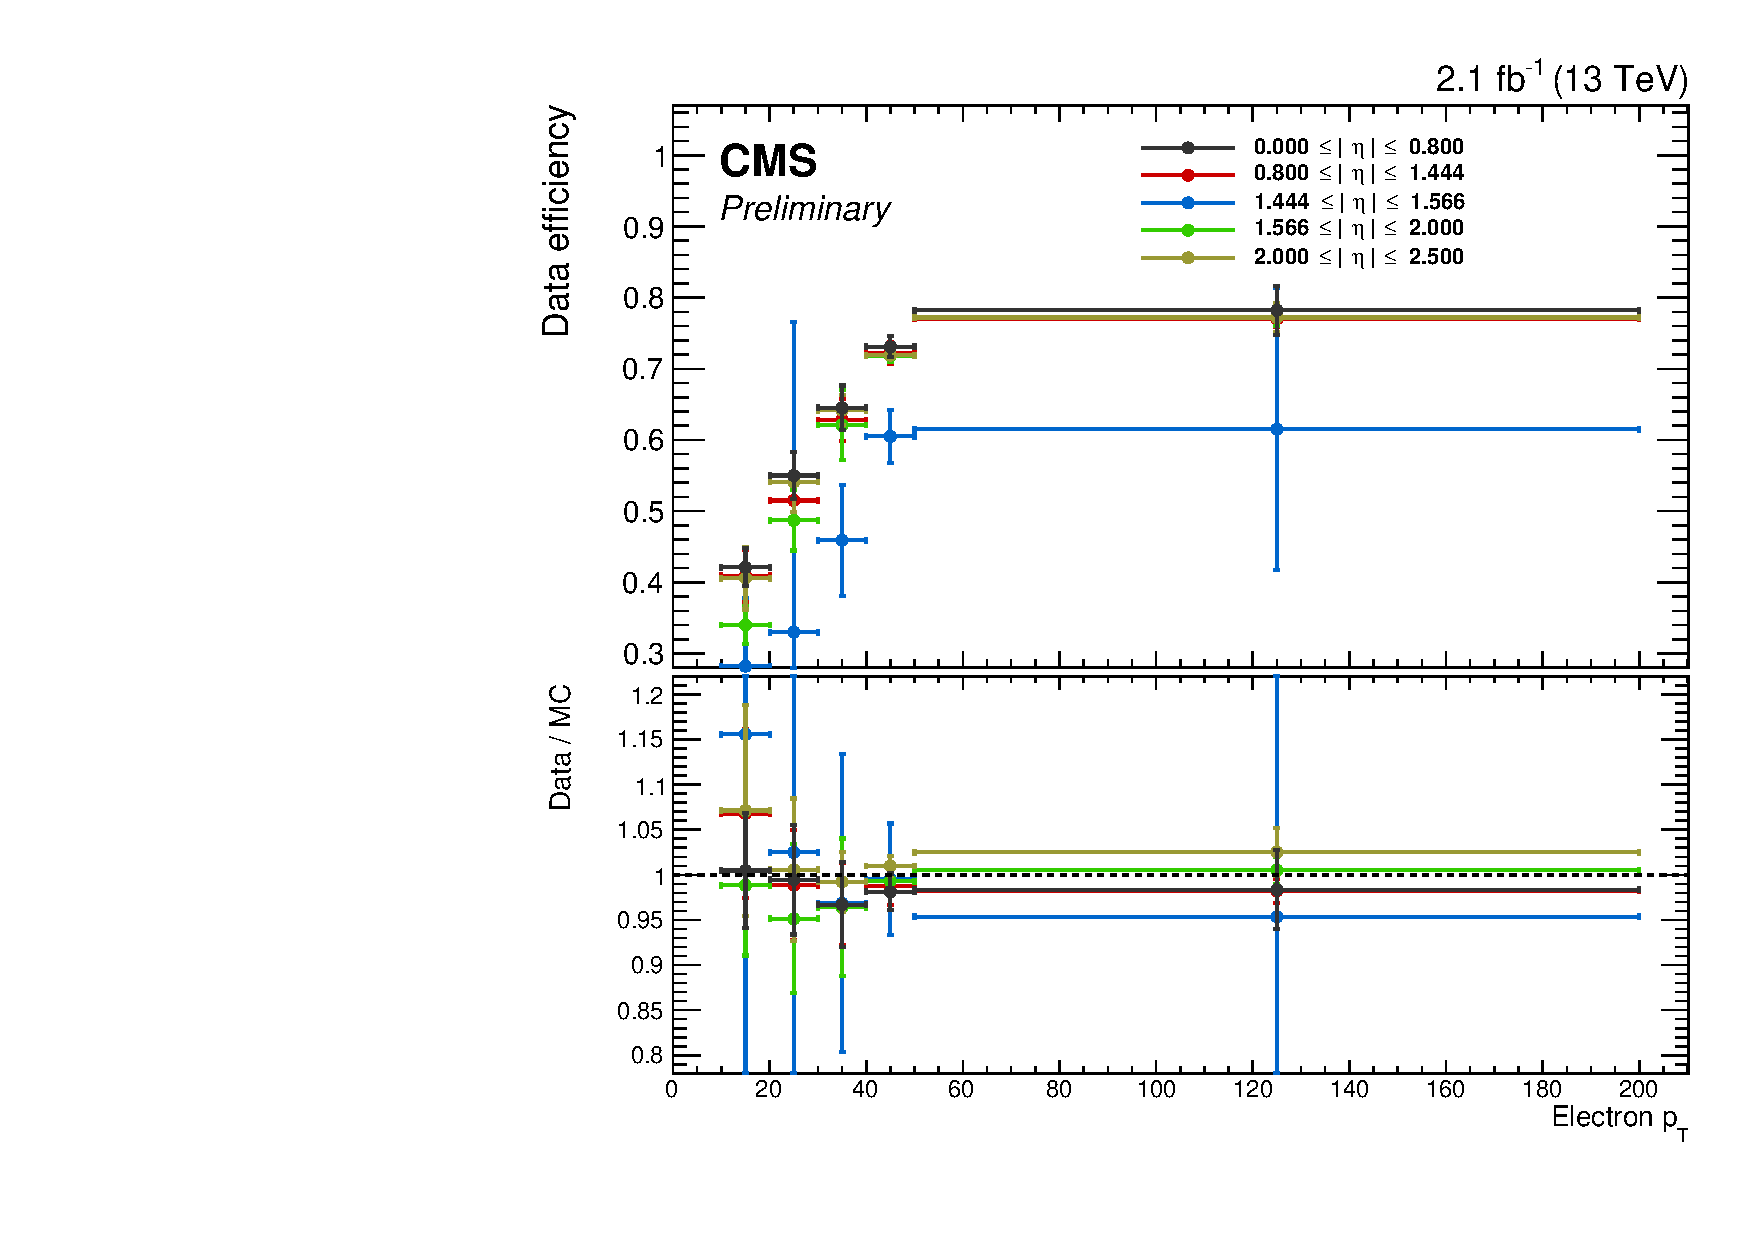
\includegraphics[width=0.5\textwidth]{images/effEleIdIso.pdf}
\caption{Typical electron identification and isolation efficiencies in data (top panel) and data/simulation scale factor (bottom panel), as a function of the electron \pt and for different $\eta$ bins.}\label{fig:eleIdIso}
\end{figure}
	
	
	
	
	
	
\subsection{Lepton trigger efficiency}\label{sec:trigeff}
Analyses that involve leptons in the final state generally select the interesting events using lepton triggers. For instance, the \hwwllnn channel is characterized by the presence of two leptons in the final state, thereby both single lepton and double lepton triggers are used. The lepton triggers at the HLT level are characterized by \pt thresholds above which the trigger efficiency is very high (plateau region). Nevertheless, the trigger efficiency as a function of the lepton \pt is not a step function, but is characterized by a steep increase of the efficiency around the \pt threshold (turn-on region). The simulated samples thus need to be corrected in order to properly take into account the trigger efficiency. This can be achieved in two ways: including the HLT trigger in the event simulation or calculating the trigger efficiency in data and then applying it on simulated events. Several analyses, such as those related to the \hwwllnn channel, opt for the second approach.

The trigger efficiency for single and double lepton triggers is calculated in bins of $\eta$ and \pt using a Tag and Probe technique similar to the one described in Sec.~\ref{sec:lepIdIsoEff}, separately for muons and electrons. Since the triggered events arise from a mixture of two different triggers, the combined efficiency has to be computed and applied to simulated samples as an event weight. In the following, the approach used in the \hwwllnn analyses is described.

The event efficiency $\varepsilon_\mathrm{ev}$ for an event with two leptons to pass the single lepton trigger is given by the following formula:
\begin{equation}\label{eq:single_trigg}
\varepsilon_\mathrm{ev} = 1 - (1-\varepsilon_{S,\ell1})\cdot(1-\varepsilon_{S,\ell2})\quad,
\end{equation}

\noindent where $\varepsilon_{S,\ell1}$ and $\varepsilon_{S,\ell2}$ are the efficiencies for the leading and subleading lepton to pass the single lepton trigger. In other words, the dilepton event passes the single lepton trigger if either one of the two leptons passes the single lepton trigger, excluding the cases for which both leptons pass the trigger. 

For double lepton triggers the efficiency is calculated separately for each leg of the trigger. In the calculation of the efficiencies the two trigger legs are considered independent, given that the correlations are very small. The combined efficiency is then used as a kinematics-dependent weight to be applied on simulated events. The event efficiency can be written as:
\begin{equation}\label{eq:double_trigg}
\varepsilon_\mathrm{ev}  = \varepsilon_{D,\ell1}^\mathrm{lead} \cdot \varepsilon_{D,\ell2}^\mathrm{trail} + (  1 -  \varepsilon_{D,\ell1}^\mathrm{lead} \cdot \varepsilon_{D,\ell2}^\mathrm{trail})\cdot\varepsilon_{D,\ell1}^\mathrm{trail} \cdot \varepsilon_{D,\ell2}^\mathrm{lead} \quad,
\end{equation}

\noindent where $\varepsilon_{D,\ell1}^{\mathrm{lead}(trail)}$ is the efficiency of the first lepton to pass the leading (trailing) leg of the double lepton trigger, and $\varepsilon_{D,\ell2}^{\mathrm{lead}(trail)}$ is the efficiency of the second lepton to pass the leading (trailing) leg of the double lepton trigger. The final event efficiency applied to reweight the events in simulation is given by the boolean OR of the event efficiencies corresponding to the single and double lepton triggers, which using Eqs.~\eqref{eq:single_trigg} and ~\eqref{eq:double_trigg}, can be written as:
\begin{equation}
\begin{split}
\varepsilon_\mathrm{ev} & = 1 - (1-\varepsilon_{S,\ell1})\cdot(1-\varepsilon_{S,\ell2}) + \\
                     & + (1-\varepsilon_{S,\ell1})\cdot(1-\varepsilon_{S,\ell2}) \cdot \\
                     & \cdot [ \varepsilon_{D,\ell1}^\mathrm{lead} \cdot \varepsilon_{D,\ell2}^\mathrm{trail} + (  1 -  \varepsilon_{D,\ell1}^\mathrm{lead} \cdot \varepsilon_{D,\ell2}^\mathrm{trail})\cdot\varepsilon_{D,\ell1}^\mathrm{trail} \cdot \varepsilon_{D,\ell2}^\mathrm{lead} ] \quad.
\end{split}
\end{equation}

%The term that multiplies the double lepton trigger event efficiency is needed to ensure that the events passing the double lepton trigger do not pass also the single lepton trigger.



